\section{Empirical Evaluations on Machine Learning Benchmarks}
\label{sec:evaluation}

We evaluate DeXposure-FM on the DeXposure dataset through two machine learning benchmark tasks: (i) \textit{multi-step forecasting} of edge existence/weights and node TVL changes; and (ii) \textit{predictive contagion stress testing}, where we forecast future stress-test losses under counterfactual shocks. Section~\ref{sec:econ} then translates these predictive outputs into macroprudential monitoring tools (systemic importance, spillovers, stress testing, and early warning) and validates them on historical stress events.

\subsection{Dataset and Experimental Setup}
\label{subsec:dataset}

\paragraph{Data source.}
We use the DeXposure dataset constructed from DeFiLlama API data, spanning March 2020 to August 2025 (283 weekly snapshots). Each snapshot contains protocol nodes with TVL measurements and directed edges representing credit exposures between protocols.

\paragraph{Data statistics.}
Table~\ref{tab:data-stats} summarizes the dataset characteristics. The network exhibits high edge persistence (mean overlap ratio 98.5\%), reflecting the stable nature of DeFi protocol interconnections.

\begin{table}[t]
\centering
\small
\begin{tabular}{lr}
\hline
\textbf{Statistic} & \textbf{Value} \\
\hline
Total snapshots & 283 weeks \\
Time range & 2020-03-23 $\sim$ 2025-08-18 \\
Mean nodes per week & 5,676 \\
Mean edges per week & 30,424 \\
Mean edge overlap ratio & 98.5\% \\
Protocol categories & $\sim$15 classes \\
\hline
\end{tabular}
\caption{DeXposure dataset statistics.}
\label{tab:data-stats}
\end{table}

\paragraph{Temporal split.}
We use a two-stage evaluation protocol:

\textit{Stage 1: Model selection via walk-forward cross-validation.}
We apply expanding window walk-forward cross-validation on pre-2025 data with 15 folds. Each fold uses a minimum of 104 training weeks, 24 validation weeks (for early stopping), and 8 test weeks. The validation window is sized to ensure sufficient samples even at longer horizons: for $h=12$, we require $\geq 12$ validation weeks to construct valid forecast pairs. The window advances by 8 weeks per fold, accumulating more training data. This stage is used for hyperparameter selection and model comparison.

\textit{Stage 2: Hold-out evaluation.}
Final performance is reported on a strict 2025 hold-out set, which is never seen during training or validation:
\begin{itemize}
  \item \textbf{Training:} 2020-03-23 $\sim$ 2024-07-15 (225 weeks)
  \item \textbf{Validation:} 2024-07-22 $\sim$ 2024-12-30 (24 weeks, for early stopping)
  \item \textbf{Test:} 2025-01-06 $\sim$ 2025-08-18 (33 weeks, strict hold-out)
\end{itemize}
Stage 1 is used for hyperparameter tuning; all results reported in this paper are from Stage 2 hold-out evaluation.

\paragraph{Forecast horizons vs. CV windows.}
The 8-week CV window controls how the temporal folds slide; within each window, the model predicts at multiple forecast horizons $h \in \{1, 4, 8, 12\}$ weeks ahead. These are orthogonal: the CV window determines sample collection, while $h$ determines how far into the future each prediction extends.

\paragraph{Models compared.}
We compare three approaches:
\begin{enumerate}
  \item \textbf{GraphPFN:} Pre-trained GraphPFN encoder with frozen weights; only task-specific prediction heads are trained (linear probe).
  \item \textbf{DeXposure-FM:} Pre-trained GraphPFN encoder with end-to-end fine-tuning using differential learning rates.
\item \textbf{ROLAND:} Representative temporal GNN baseline with a 2-layer GCN encoder (hidden\_dim=64, out\_dim=32) and GRU temporal updates for recurrent state propagation, trained from scratch. Uses the same optimizer (Adam), learning rate ($5 \times 10^{-4}$), and training schedule as DeXposure-FM.
\end{enumerate}

\subsection{Task I: Multi-step Forecasting}
\label{subsec:forecast}

\subsubsection{Implementation Details}
\label{subsubsec:task1-impl}
We evaluate forecasts at horizons $h \in \{1, 4, 8, 12\}$ weeks for:
\begin{enumerate}
  \item \textbf{Edge existence:} Binary prediction of whether edge $(p,q)$ exists at $t+h$.
  \item \textbf{Edge weight:} Regression on log-scaled edge weight for existing edges.
  \item \textbf{Node TVL change:} Regression on $\Delta_{p,t+h} = \log(1+\text{TVL}_{t+h}) - \log(1+\text{TVL}_t)$.
\end{enumerate}

\noindent We report AUPRC/AUROC for edge existence and MAE/RMSE for edge weights and node $\Delta$TVL on log-scaled values.

\subsubsection{Empirical Results}
\label{subsubsec:task1-results}
For edge existence, we report AUPRC (area under precision-recall curve) and AUROC. For edge weight and node predictions, we report MAE and RMSE on log-scaled values.

Table~\ref{tab:main-results} presents the main forecasting results on the 2025 hold-out test set.
%% [Updated to h={1,4,8,12} with complete DeXposure-FM results from GPU server experiments]

\begin{table}[t]
\centering
\small
\setlength{\tabcolsep}{4pt}
\begin{tabular}{llcccccc}
\hline
& & \multicolumn{2}{c}{\textbf{Edge Exist}} & \multicolumn{2}{c}{\textbf{Edge Weight}} & \multicolumn{2}{c}{\textbf{Node $\Delta$TVL}} \\
\textbf{Model} & $h$ & AUROC & AUPRC & MAE & RMSE & MAE & RMSE \\
\hline
\multirow{4}{*}{DeXposure-FM}
& 1 & \textbf{0.995} & \textbf{0.972} & \textbf{2.465} & \textbf{3.388} & \textbf{0.056} & \textbf{0.400} \\
& 4 & \textbf{0.995} & \textbf{0.973} & \textbf{2.489} & \textbf{3.424} & \textbf{0.140} & \textbf{0.680} \\
& 8 & \textbf{0.994} & \textbf{0.967} & \textbf{2.554} & \textbf{3.509} & \textbf{0.229} & \textbf{0.890} \\
& 12 & \textbf{0.993} & \textbf{0.967} & \textbf{2.648} & \textbf{3.606} & \textbf{0.286} & \textbf{1.046} \\
\hline
\multirow{4}{*}{GraphPFN}
& 1 & 0.988 & 0.938 & 3.260 & 4.383 & 0.059 & 0.401 \\
& 4 & 0.988 & 0.940 & 3.189 & 4.049 & 0.142 & 0.682 \\
& 8 & 0.987 & 0.938 & 3.169 & 4.064 & 0.215 & 0.896 \\
& 12 & 0.986 & 0.936 & 3.136 & 4.130 & 0.324 & 1.056 \\
\hline
\multirow{4}{*}{ROLAND}
& 1 & 0.961 & 0.865 & 3.240 & 4.264 & 0.060 & 0.403 \\
& 4 & 0.962 & 0.868 & 3.242 & 4.162 & 0.141 & 0.684 \\
& 8 & 0.961 & 0.867 & 3.213 & 4.180 & 0.221 & 0.895 \\
& 12 & 0.961 & 0.866 & 3.195 & 4.177 & 0.279 & 1.058 \\
\hline
\multirow{4}{*}{Persistence}
& 1 & 0.763 & 0.604 & 2.487 & 4.296 & 0.057 & 0.403 \\
& 4 & 0.782 & 0.635 & 2.372 & 4.138 & 0.138 & 0.685 \\
& 8 & 0.749 & 0.580 & 2.618 & 4.400 & 0.213 & 0.899 \\
& 12 & 0.762 & 0.603 & 2.541 & 4.304 & 0.272 & 1.065 \\
\hline
\end{tabular}
\caption{Multi-step forecasting results on 2025 hold-out test set at horizons $h \in \{1,4,8,12\}$ weeks. DeXposure-FM = Finetuned Foundation Model, GraphPFN = Graph Prior Fitted Network with Frozen weights. \textit{Persistence} = naive baseline predicting $\hat{A}_{t+h} = A_t$, $\hat{W}_{t+h} = W_t$.}
\label{tab:main-results}
\end{table}

\paragraph{Key findings.}
\begin{enumerate}
  \item \textbf{Edge existence substantially exceeds persistence:} All models dramatically outperform the naive persistence baseline (AUPRC 0.58--0.64) that simply predicts ``last week's graph.'' DeXposure-FM achieves AUPRC 0.967--0.973, representing a 52--67\% relative improvement over persistence. This confirms the models learn meaningful temporal dynamics beyond network inertia.
  \item \textbf{Edge weight matches persistence:} Surprisingly, edge weight prediction shows no improvement over the persistence baseline (MAE 2.37--2.62). DeXposure-FM achieves MAE 2.465--2.648, comparable to or slightly worse than persistence at some horizons. This indicates that learned models excel at predicting \textit{which} edges exist, but predicting \textit{how much} exposure flows through them remains fundamentally challenging---the best strategy is often ``predict last week's value.''
  \item \textbf{Model value is in link prediction:} The primary value of DeXposure-FM lies in edge existence prediction. Compared to learned baselines, it achieves 3--8\% AUPRC improvement over GraphPFN and 10--12\% over ROLAND, while maintaining comparable weight and node predictions.
  \item \textbf{Node prediction degrades with horizon:} Node TVL change prediction degrades as expected: DeXposure-FM MAE increases from 0.056 ($h=1$) to 0.286 ($h=12$), matching persistence (0.057--0.272) at all horizons.
\end{enumerate}

\subsection{Task II: Financial Stability Analysis}
\label{subsec:stability}

This task evaluates whether forward-looking network forecasts translate into forward-looking \emph{stress test} forecasts. Specifically, we compare contagion losses computed on the model-predicted future network $\hat{G}_{t+h}$ with losses on the realized future network $G_{t+h}$, under fixed counterfactual shock definitions.

\subsubsection{Implementation Details}
\label{subsubsec:task2-impl}
We use a fixed DeXposure-FM forecaster trained on the pre-2025 training period and early-stopped on the pre-2025 validation period (Stage 2 in Section~\ref{subsec:dataset}). We then evaluate on the strict 2025 hold-out set without re-estimation during the test period. Each test week provides an origin $t$, yielding multiple out-of-sample pairs $(t,t+h)$ for horizons $h\in\{1,4,8,12\}$. To handle protocol entry/exit, all comparisons are computed on the common node set $V_t \cap V_{t+h}$.

Stress-test losses are computed using a DebtRank-style contagion simulator (Section~\ref{subsubsec:contagion}) under three scenarios: (i) \textbf{Top protocol shock} (50\% TVL loss to the largest protocol), (ii) \textbf{Top-5 protocols shock} (30\% TVL loss to the top-5 protocols), and (iii) \textbf{Bridge sector shock} (100\% TVL loss to bridge protocols). For each $(t,t+h)$, we run the simulator on three graphs: the observed network at $t$ (persistence baseline), the predicted network $\hat{G}_{t+h}$, and the realized network $G_{t+h}$.

Because the DeFi exposure network is highly persistent (Table~\ref{tab:data-stats}), the persistence baseline is difficult to beat on average. To surface policy-relevant headroom, we also evaluate an \emph{advantage regime}: the \textbf{worst 20\%} of test cases under persistence (largest baseline absolute errors within each horizon, pooled across shock scenarios). We summarize performance with $\Delta \mathrm{MAE}=\mathrm{MAE}(\text{baseline})-\mathrm{MAE}(\text{model})$, where positive values indicate improvement over persistence.

\subsubsection{Empirical Results}
\label{subsubsec:task2-results}
Figure~\ref{fig:contagion-comparison} shows the three-way comparison (baseline vs.\ model vs.\ realized) and Figure~\ref{fig:contagion-advantage} visualizes $\Delta\mathrm{MAE}$ in both the overall population and the worst-20\% tail. Table~\ref{tab:contagion-advantage} reports horizon-level summary statistics.

Across horizons, persistence remains strong on average ($\Delta\mathrm{MAE}(\text{all})<0$), but DeXposure-FM consistently improves performance in the tail ($\Delta\mathrm{MAE}(\text{worst20\%})>0$), with worst20\% win rates of 83--100\%. These gains are concentrated in bridge-sector shocks (Figure~\ref{fig:contagion-advantage}), consistent with non-stationary exposure reallocation through cross-chain liquidity conduits. Section~\ref{sec:econ} further examines how these forecasts support macroprudential tools such as forward-looking risk metric monitoring and early warning event studies.

\begin{figure}[t]
\centering
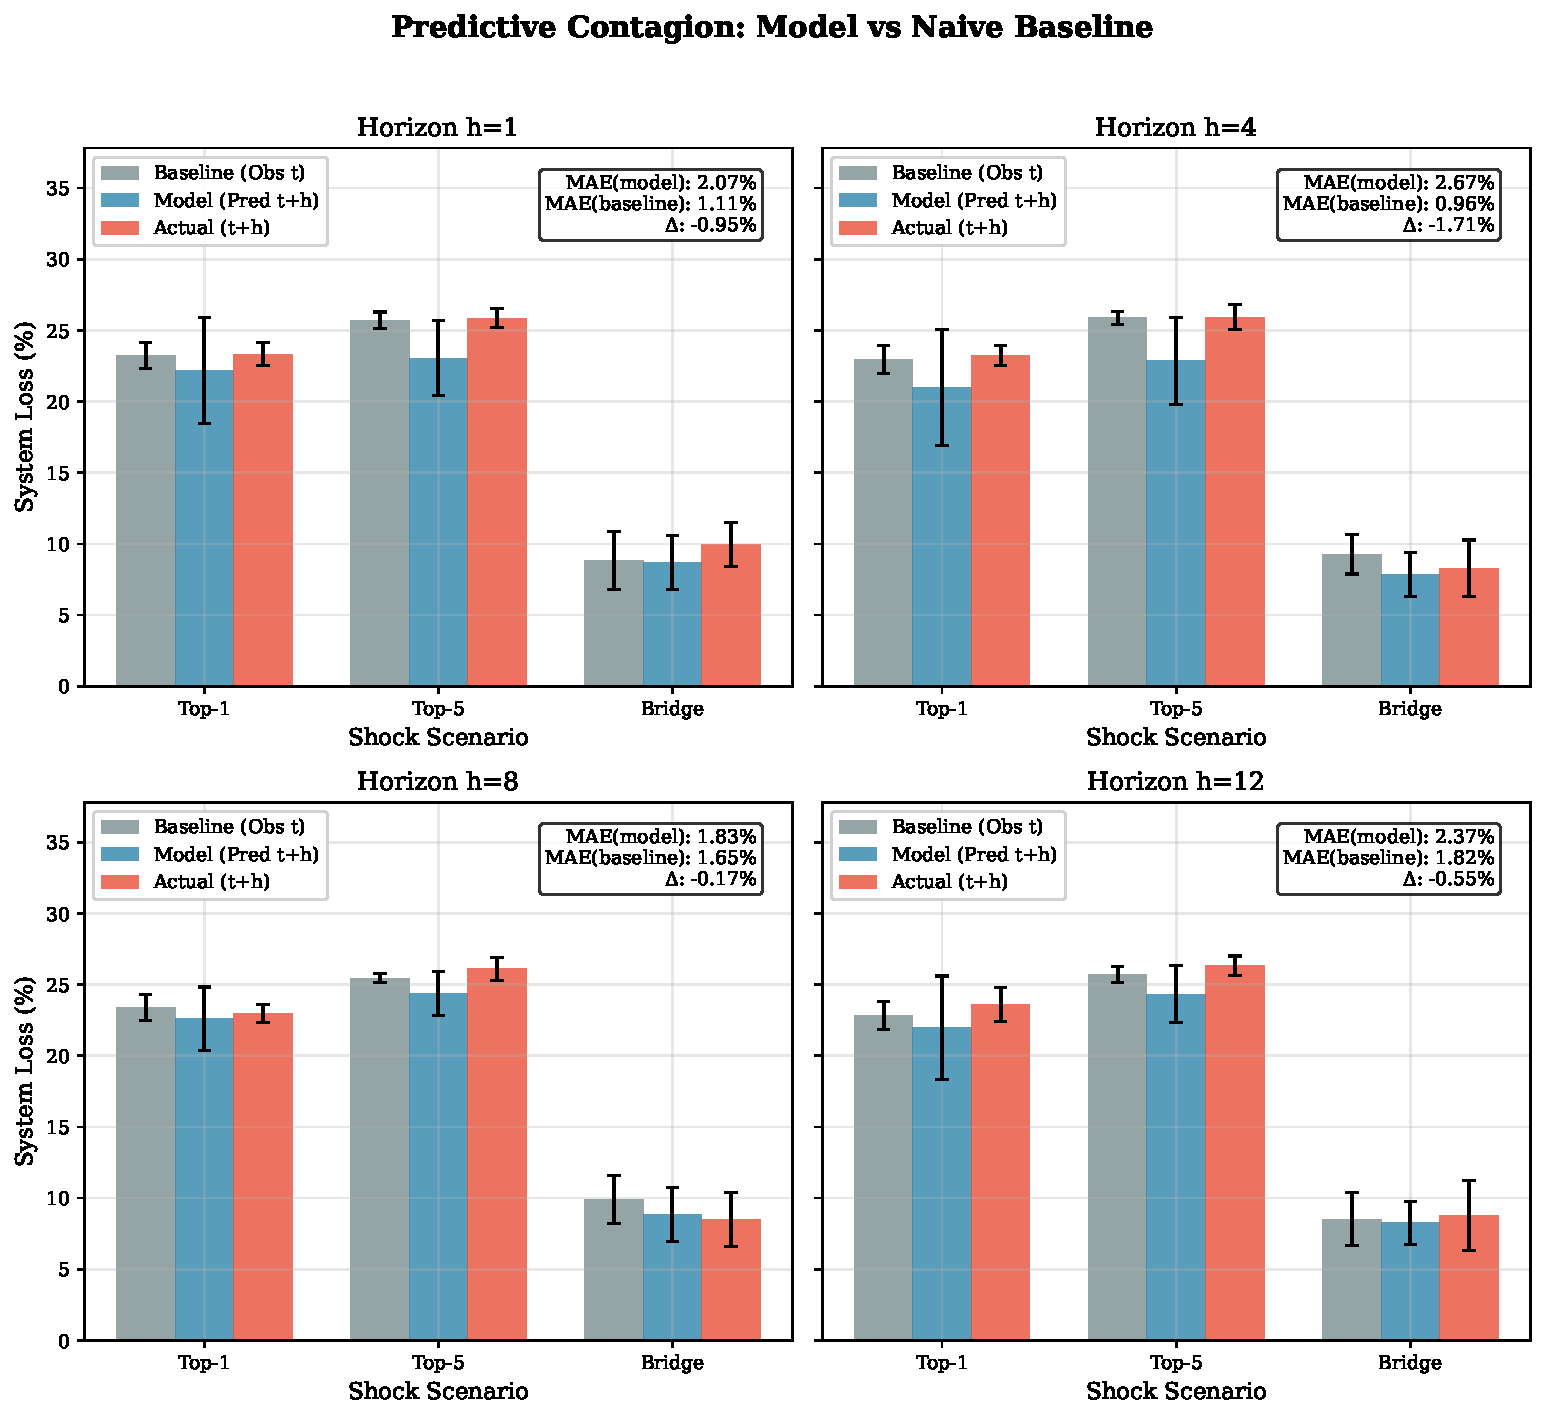
\includegraphics[width=0.95\textwidth]{figures/fig_contagion_comparison.pdf}
\caption{Predictive contagion stress testing (Task II). We compare system loss (\%) under identical shocks when running the contagion simulator on the observed network at time $t$ (persistence baseline), the model-predicted network $\hat{G}_{t+h}$, and the realized future network $G_{t+h}$.}
\label{fig:contagion-comparison}
\end{figure}

\begin{figure}[t]
\centering
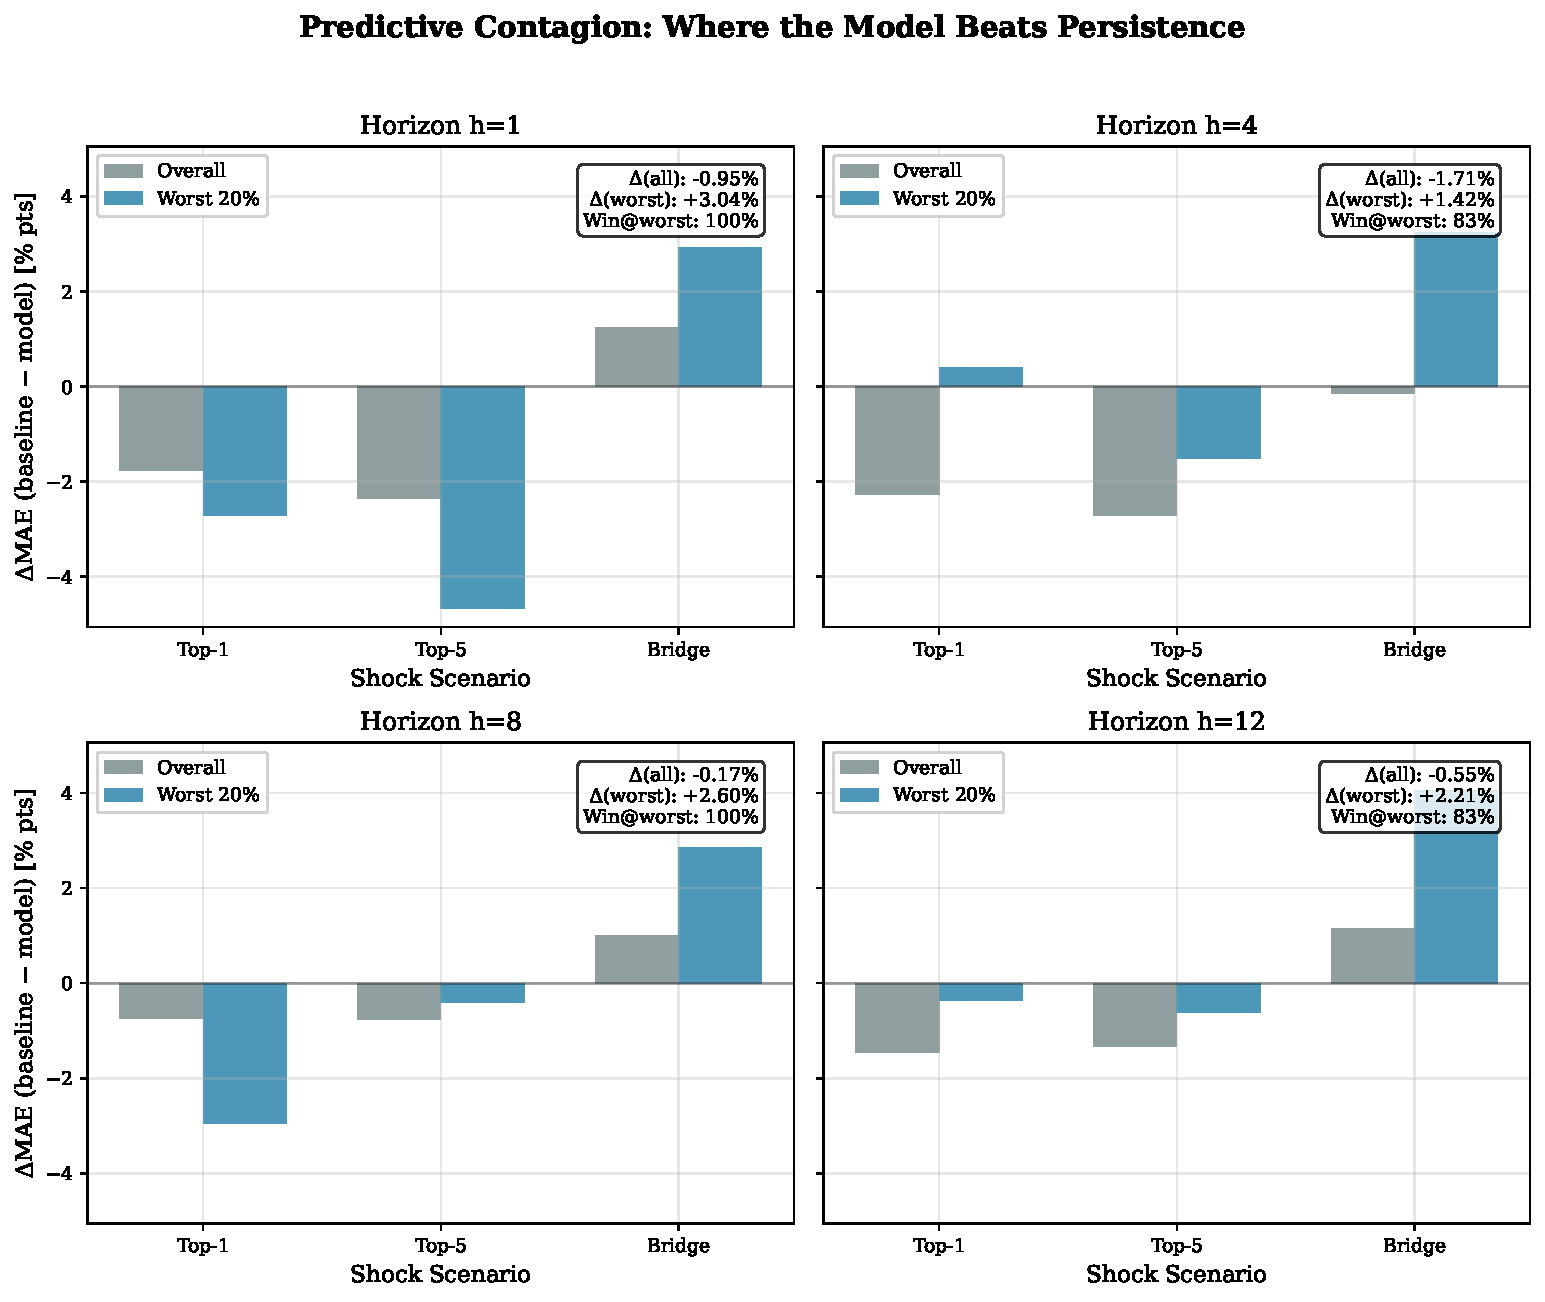
\includegraphics[width=0.95\textwidth]{figures/fig_contagion_advantage.pdf}
\caption{Advantage regimes for forward-looking stress testing. Bars report $\Delta\mathrm{MAE}=\mathrm{MAE}(\text{baseline})-\mathrm{MAE}(\text{model})$ in system loss (\% points). ``Overall'' is the full test set; ``Worst 20\%'' restricts to the 20\% largest baseline errors (tail regime). Positive values indicate DeXposure-FM outperforms persistence, highlighting where a foundation model adds value under non-stationarity.}
\label{fig:contagion-advantage}
\end{figure}

\begin{table}[t]
\centering
\small
\setlength{\tabcolsep}{6pt}
\begin{tabular}{lccc}
\hline
Horizon $h$ & $\Delta\mathrm{MAE}(\text{all})$ & $\Delta\mathrm{MAE}(\text{worst20\%})$ & Win rate (worst20\%) \\
\hline
1  & $-0.95$ & $+3.04$ & 100\% \\
4  & $-1.71$ & $+1.42$ & 83\% \\
8  & $-0.17$ & $+2.60$ & 100\% \\
12 & $-0.55$ & $+2.21$ & 83\% \\
\hline
\end{tabular}
\caption{Predictive stress testing summary (2025 hold-out). $\Delta\mathrm{MAE}$ is measured in system-loss percentage points. Worst20\% selects the 20\% largest persistence-baseline errors within each horizon (pooled across shock scenarios). ``Win rate'' is the fraction of worst20\% cases where the model has lower absolute error than persistence.}
\label{tab:contagion-advantage}
\end{table}
